\documentclass{beamer}

% opacity bugfix: see http://tug.org/pipermail/pdftex/2007-December/007480.html
\pdfpageattr {/Group << /S /Transparency /I true /CS /DeviceRGB>>}

\usepackage[utf8]{inputenc}
\usepackage[OT1]{fontenc}

\usepackage{tikz}
\usetikzlibrary{%
   arrows,%
   calc,%
   fit,%
   patterns,%
   plotmarks,%
   shapes.geometric,%
   shapes.misc,%
   shapes.symbols,%
   shapes.arrows,%
   shapes.callouts,%
   shapes.multipart,%
   shapes.gates.logic.US,%
   shapes.gates.logic.IEC,%
   er,%
   automata,%
   backgrounds,%
   chains,%
   topaths,%
   trees,%
   petri,%
   mindmap,%
   matrix,%
   calendar,%
   folding,%
   fadings,%
   through,%
   patterns,%
   positioning,%
   scopes,%
   decorations.fractals,%
   decorations.shapes,%
   decorations.text,%
   decorations.pathmorphing,%
   decorations.pathreplacing,%
   decorations.footprints,%
   decorations.markings,%
   shadows}
\usepackage{animate}
\usepackage{amssymb, amsmath, amsfonts, enumerate}
%\usepackage{bbold}
\newcommand\hmmax{0}
\usepackage{bm}
%\usepackage{dsfont}
\usepackage{pxfonts}
\usepackage{xcolor}
\usepackage{url}

\usepackage[backend=bibtex,style=authoryear,dashed=false]{biblatex}
\addbibresource{../bib/lundrefs.bib}
%\renewcommand{\bibfont}{\normalfont\scriptsize}
\setlength{\bibhang}{3ex}

\usepackage{hyperref}

\usetheme[official=false,department=none]{tue2008}
%\usefonttheme{default}


%\usetheme[secheader]{Boadilla}
%\setbeamercovered{transparent}
%\setbeamercovered{invisible}
%\setbeamertemplate{navigation symbols}{}
%\setbeamertemplate{bibliography item}[text] % numbered references
%\useoutertheme{infolines}
%\setbeamertemplate{headline}{}
%\setbeamertemplate{footline}{\hspace*{5mm}\hfill\insertframenumber\hspace*{5mm}\vspace{3mm}}
%\setbeamercolor{alerted text}{fg=orange!80!black}

% ------------------------------------------------------------------------------

\newcommand{\vcenterbox}[1]{\ensuremath{\vcenter{\hbox{#1}}}}
%
\newcommand{\reals}{\mathbb{R}}
\newcommand{\posreals}{\reals_{>0}}
\newcommand{\posrealszero}{\reals_{\ge 0}}
\newcommand{\naturals}{\mathbb{N}}

\newcommand{\dd}{\,\mathrm{d}}

\newcommand{\mbf}[1]{\mathbf{#1}}
\newcommand{\bs}[1]{\boldsymbol{#1}}
\renewcommand{\vec}[1]{{\bm#1}}

\newcommand{\uz}{^{(0)}} % upper zero
\newcommand{\un}{^{(n)}} % upper n
\newcommand{\ui}{^{(i)}} % upper i
\newcommand{\uell}{^{(\ell)}} % upper ell

\newcommand{\ul}[1]{\underline{#1}}
\newcommand{\ol}[1]{\overline{#1}}

\newcommand{\Rsys}{R_\text{sys}}
\newcommand{\lRsys}{\ul{R}_\text{sys}}
\newcommand{\uRsys}{\ol{R}_\text{sys}}

\newcommand{\Fsys}{F_\text{sys}}
\newcommand{\lFsys}{\ul{F}_\text{sys}}
\newcommand{\uFsys}{\ol{F}_\text{sys}}

\def\Tsys{T_\text{sys}}

\newcommand{\E}{\operatorname{E}}
\newcommand{\V}{\operatorname{Var}}
\newcommand{\sd}{\operatorname{sd}}

\newcommand{\wei}{\operatorname{Wei}} % Weibull Distribution
\newcommand{\ig}{\operatorname{IG}}   % Inverse Gamma Distribution
\newcommand{\ber}{\operatorname{Bernoulli}} 
\newcommand{\bin}{\operatorname{Binomial}}
\newcommand{\be}{\operatorname{Beta}} 
\newcommand{\bebin}{\operatorname{Beta-binomial}}
\newcommand{\norm}{\operatorname{N}}

\def\then{{\structure{$\rule[0.35ex]{2ex}{0.5ex}\!\!\!\blacktriangleright$}}}
\def\play{{\structure{$\blacktriangleright$}}}
\def\gplus{{\structure{\rule[0.45ex]{1.4ex}{0.4ex}\hspace{-0.9ex}\rule[0.0ex]{0.4ex}{1.3ex}\hspace{0.5ex}}}}
\def\gminus{{\structure{\rule[0.45ex]{1.4ex}{0.4ex}}}}


\def\yz{y\uz}
\def\yn{y\un}
%\def\yi{y\ui}
\newcommand{\yfun}[1]{y^{({#1})}}
\newcommand{\yfunl}[1]{\ul{y}^{({#1})}}
\newcommand{\yfunu}[1]{\ol{y}^{({#1})}}

\def\ykt{y_{k,t}}

\def\ykz{y\uz_k}
\def\ykn{y\un_k}

\def\yktz{y\uz_{k,t}}
\def\yktn{y\un_{k,t}}

\def\yzl{\ul{y}\uz}
\def\yzu{\ol{y}\uz}
\def\ynl{\ul{y}\un}
\def\ynu{\ol{y}\un}
\def\yil{\ul{y}\ui}
\def\yiu{\ol{y}\ui}

\def\ykzl{\ul{y}\uz_k}
\def\ykzu{\ol{y}\uz_k}
\def\yknl{\ul{y}\un_k}
\def\yknu{\ol{y}\un_k}

\def\yktzl{\ul{y}\uz_{k,t}}
\def\yktzu{\ol{y}\uz_{k,t}}
\def\yktnl{\ul{y}\un_{k,t}}
\def\yktnu{\ol{y}\un_{k,t}}


\def\nz{n\uz}
\def\nn{n\un}
%\def\ni{n\ui}
\newcommand{\nfun}[1]{n^{({#1})}}
\newcommand{\nfunl}[1]{\ul{n}^{({#1})}}
\newcommand{\nfunu}[1]{\ol{n}^{({#1})}}

\def\nkz{n\uz_k}
\def\nkn{n\un_k}
\newcommand{\nkzfun}[1]{n\uz_{#1}}

\def\nkt{n_{k,t}}

\def\nktz{n\uz_{k,t}}
\def\nktn{n\un_{k,t}}


\def\nzl{\ul{n}\uz}
\def\nzu{\ol{n}\uz}
\def\nnl{\ul{n}\un}
\def\nnu{\ol{n}\un}
\def\nil{\ul{n}\ui}
\def\niu{\ol{n}\ui}

\def\nkzl{\ul{n}\uz_k}
\def\nkzu{\ol{n}\uz_k}
\def\nknl{\ul{n}\un_k}
\def\nknu{\ol{n}\un_k}

\def\nktzl{\ul{n}\uz_{k,t}}
\def\nktzu{\ol{n}\uz_{k,t}}
\def\nktnl{\ul{n}\un_{k,t}}
\def\nktnu{\ol{n}\un_{k,t}}

\def\taut{\tau(\vec{t})}
\def\taux{\tau(\vec{x})}
\def\ttau{\tilde{\tau}}
\def\ttaut{\ttau(\vec{t})}
\def\ttaux{\ttau(\vec{x})}

\def\MZ{\mathcal{M}\uz}
\def\MN{\mathcal{M}\un}

\def\MkZ{\mathcal{M}\uz_k}
\def\MkN{\mathcal{M}\un_k}

\def\MktZ{\mathcal{M}\uz_{k,t}}
\def\MktN{\mathcal{M}\un_{k,t}}

\def\PZ{\Pi\uz}
\def\PN{\Pi\un}

\def\PkZ{\Pi\uz_k}
\def\PkN{\Pi\un_k}
\newcommand{\PZi}[1]{\Pi\uz_{#1}}

\def\PktZ{\Pi\uz_{k,t}}
\def\PktN{\Pi\un_{k,t}}
\newcommand{\PtZi}[1]{\Pi\uz_{#1,t}}
\newcommand{\PkZi}[1]{\Pi\uz_{k,#1}}

\newcommand{\az}{\alpha\uz}
\newcommand{\an}{\alpha\un}
\newcommand{\bz}{\beta\uz}
\newcommand{\bn}{\beta\un}


\def\blau#1{{\color{tuegreen}#1}}
\def\rot#1{{\color{tuered}#1}}
\def\gruen#1{{\color{tueblue}#1}}

\def\yzr{\rot{\yz}}
\def\ynr{\rot{\yn}}
\def\byzr{\rot{\byz}}
\def\bynr{\rot{\byn}}
\def\yzor{\rot{y\uz_1}}
\def\yzjr{\rot{y\uz_j}}
\def\yzkr{\rot{y\uz_k}}
\def\yzlr{\rot{\yzl}}
\def\yzur{\rot{\yzu}}
\def\ynjr{\rot{y\un_j}}
\def\ynlr{\rot{\ynl}}
\def\ynur{\rot{\ynu}}
\def\yzjlr#1{\rot{\ul{y}\uz_#1}}
\def\yzjur#1{\rot{\ol{y}\uz_#1}}


\def\nzg{\gruen{\nz}}
\def\nng{\gruen{\nn}}
\def\nzlg{\gruen{\nzl}}
\def\nzug{\gruen{\nzu}}
\def\nnlg{\gruen{\nnl}}
\def\nnug{\gruen{\nnu}}

\def\psib{\blau{\psi}}
\def\bpsib{\blau{{b}(\psi)}}


% ------------ shading start
\newsavebox{\tempbox}
\newcommand\leftrightshading[3]{%
  \begin{tikzfadingfrompicture}[name=inputtext]
    \node [text=white] {#1};
  \end{tikzfadingfrompicture}
  \begin{lrbox}{\tempbox}%
    \begin{tikzpicture}
      \node [text=white,inner sep=0pt,outer sep=0pt] (textnode) {#1};
      \shade[path fading=inputtext,fit fading=false,left color=#2,right color=#3]
      (textnode.south west) rectangle (textnode.north east);
    \end{tikzpicture}%
  \end{lrbox}
  % Now we use the fading in another picture:
  \usebox\tempbox{}%
}
% ------------ shading end


%\def\PZc{\mathrm I\!\Pi\uz}
\def\PZc{\leftrightshading{$\mathrm I\!\Pi\uz$}{blue}{red}}
%\def\PNc{\PN}
\def\PNc{\leftrightshading{$\mathrm I\!\Pi\un$}{blue}{red}}



%%\def\blau#1{{\color{lmugreen2}#1}}
%\def\rot#1{{\color{red}#1}}
%\def\gruen#1{{\color{blue}#1}}


\def\tnow{t_\text{now}}
\def\tpnow{t^+_\text{now}}

\newcommand{\comp}[1]{\raisebox{-1mm}{\tikz{\node[%type1
rectangle,rounded corners=0mm,draw,fill=tuepmsgreen!70,thick,inner sep=0pt,minimum size=4mm]{#1};}}}

\newcommand{\cyansec}[1]{\textcolor{tuecyan}{\large\bf #1}}
\newcommand{\cyanalert}[1]{\textcolor{tuecyan}{#1}}
\newcommand{\bluesec}[1]{\textcolor{tueblue}{\large\bf #1}}
\newcommand{\bluealert}[1]{\textcolor{tueblue}{#1}}

\setbeamertemplate{itemize item}{\tiny\raise1.5pt\hbox{\color{tueblue}$\blacktriangleright$}}

% ------------------------------------------------------------------------------


\title{Bayesian Inference and Prior-Data Conflict}

\author{Gero Walter}
\institute{ Eindhoven University of Technology, Eindhoven, NL\\[2ex]
            \url{g.m.walter@tue.nl} \\[2ex]
            
\includegraphics[height=9mm]{logos/tuelogo} \quad
            
\includegraphics[height=9mm]{logos/dinalog-hp} }
\date{2015-12-15}

\begin{document}

\frame{
\titlepage
}

\addtocounter{framenumber}{-1} 

\frame{
\frametitle{Bayesian Inference}
\begin{center}
\begin{tikzpicture} % l b r t
\uncover<1>{\node at (0,0) {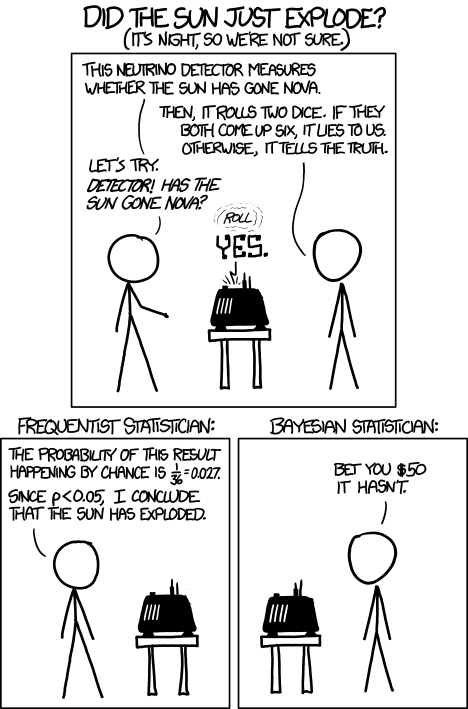
\includegraphics[height=0.9\textheight,trim = 0 300 0 0, clip]{frequentists_vs_bayesians}};}
\uncover<2>{\node at (0,0) {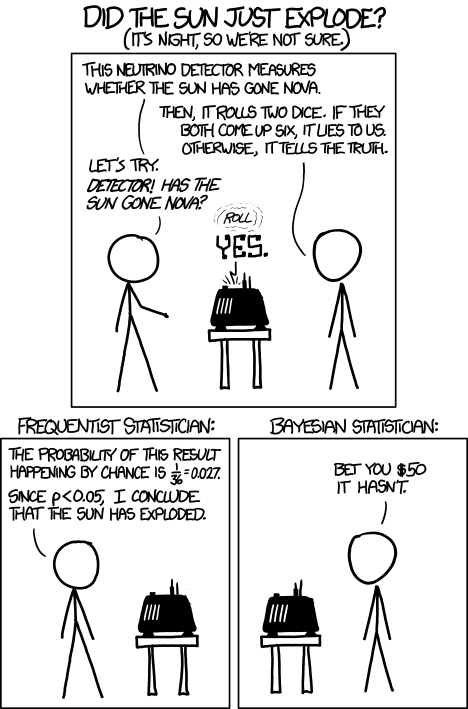
\includegraphics[width=0.9\textwidth,trim = 0 0 0 410, clip]{frequentists_vs_bayesians}};}
\end{tikzpicture}
{\footnotesize \url{https://xkcd.com/1132}}
\end{center}
}


\frame{
\frametitle{Bayesian Inference}
\begin{align*}
\begin{array}{ccccl}
\uncover<1->{\text{expert info}        & + & \text{data}                & \to & \text{complete picture} \\[1.5ex]}
\uncover<2->{\text{prior distribution} & + & \text{sample distribution} & \to & \text{posterior distribution} \\[1.5ex]
 f(\theta) & \times & f(\vec{x} \mid \theta) & \propto & p(\theta \mid \vec{x}) \\
 & & & & \qquad\text{\bluealert{\play\ Bayes' Rule}} \\}
%\uncover<3->{\downarrow & & \downarrow & & \hspace*{3ex} \downarrow \\
\uncover<4->{\text{Beta prior}}   & & \uncover<3->{\text{Binomial}}         & & \uncover<5->{\text{Beta posterior}} \\
\uncover<4->{}                    & & \uncover<3->{\text{distribution}}     & & \uncover<5->{\qquad \text{\bluealert{\play\ conjugacy}}}\\[1ex]
\uncover<4->{p \sim \be(\az,\bz)} & & \uncover<3->{s \mid p \sim \bin(n,p)} & & \uncover<5->{p \mid s \sim \be(\an,\bn)}
\end{array}
\end{align*}
\uncover<6->{\begin{itemize}
\item conjugate prior makes learning about parameter tractable,\\  %posterior distribution
      just update hyperparameters:\quad $\az \to \an$, $\bz \to \bn$
\item closed form for some inferences: $\E[p] = \frac{\an}{\an+\bn}$
\end{itemize}}
}

\frame{
\frametitle{Prior-Data Conflict}
\uncover<1->{What if expert information and data tell different stories?\\[1ex]}
\uncover<2->{%
\begin{block}{Prior-Data Conflict}
\begin{itemize}
\item \emph{informative prior beliefs} and \emph{trusted data}\\ %\rule{0ex}{3ex}\\
(sampling model correct, no outliers, etc.) are in conflict%\\%[2ex]
\item ``[\ldots] the prior [places] its mass primarily on distributions
in the sampling model for which the observed data is surprising''\\
\parencite{2006:evans}
\item there are not enough data to overrule the prior
\end{itemize}
\end{block}}
%\uncover<3->{}
%\uncover<4->{\play\ reparametrization helps to understand effect of prior-data conflict:\\}
}

\frame{\frametitle{Prior-Data Conflict: Example}

%Example Beta-Binom, show point, line, rectangle
\begin{itemize}[<+->]
\item Bernoulli observations: 0/1 observations (failure/success)
\item given: a set of $n$ observations and strong prior information
\item we are, e.g., interested in probability for success in next trial
\end{itemize}
\uncover<4->{
\begin{block}{Beta-Binomial Model}
\begin{tabular}{r|lcl}
data :           & $s \mid p$        & $\sim$ & $\bin(n,p)$   \\[0.5ex]
conjugate prior: & $p \mid \az, \bz$ & $\sim$ & $\be(\az,\, \bz)$  \\[0.5ex]
\cline{1-4}
posterior:       & $p \mid \an, \bn$ & $\sim$ & $\be(\an,\, \bn)$\rule{0ex}{2.5ex}
%\quad ($\frac{\tau(\x)}{n} = \frac{s}{n}$)\rule{0ex}{2.5ex}
\end{tabular}
\end{block}
where $s$ = number of successes in the $n$ observed trials}
}

\frame{
\frametitle{Reparametrisation of the Beta}
\uncover<1->{\play\ reparametrisation helps to understand effect of prior-data conflict:\\}
\begin{tikzpicture}
[pfeil/.style={-latex', line width=1mm, color=tuered, shorten <=1mm},
 cyanrand/.style={rounded corners, text centered, draw=tuecyan!50, inner sep=1mm, line width=0.7mm},
 redbrace/.style={draw=tuered, decoration=brace, decorate, line width=0.8mm},
 redbox/.style={text centered, draw=tuered, inner sep=1.5mm, line width=1mm}]
\uncover<1->{%
\node at (0,0.2) {\parbox[c]{\textwidth}{%
\begin{align*}
\nzg &= \az + \bz\,,
&
\yzr &= \frac{\az}{\az + \bz}\,, \quad \text{which are updated as}\\%[1.5ex]
%\\
%\end{align*}
%\intertext{%
%such that
%$\lambda \sim \ig(\nz+1,\nz\yz)$ and $\lambda\mid\mbf{t} \sim \ig(\nell+1,\nell\yell)$,
%where}%
%\begin{align*}
\nng &= \nzg + n\,, 
&
\ynr &=  \frac{\nzg}{\nzg + n} \, \yzr + \frac{n}{\nzg + n} \cdot \frac{s}{n}
\end{align*}
}};}
\uncover<2->{%
\node[cyanrand] (yz) at (-0.9,-1.9) {$\yzr = \E[p]$};
\draw [pfeil] (yz.north east) to [out= 30,in=260] ( 0.9,-0.65);
\draw [pfeil] (yz.north west) to [out=130,in=240] (-1.7,0.4);}
\uncover<3->{%
\node[cyanrand] (yn) at ( 1.4,-1.9) {$\ynr = \E[p \mid s]$};
\draw [pfeil] (yn.north)      to [out=130,in=280] (-1.4,-0.65);}
\uncover<4->{%
\node[cyanrand] (ml) at ( 4.3,-1.9) {ML estimator $\hat{p}$};
\draw [pfeil] (ml.north)      to [out=100,in=330] (3.6,-0.65);}
\uncover<5->{%
\node[cyanrand] (nz) at (-4  ,-1.9) {$\nzg =$ pseudocounts};
\draw [pfeil] (nz.north)      to [out=90,in=270] (-4.0,-0.65);
\draw [pfeil] (nz.north west) to [out=95,in=240] (-5.2, 0.5);}
\uncover<6->{%
\node[redbox] at (0,-2.8) {$\E[p \mid s]$ is a weighted average of $\E[p]$ and $\hat{p}$!};}
\uncover<7->{%
\node[redbox] at (0,-4.0) {$\V[p \mid s] = \dfrac{\ynr (1-\ynr)}{\nng + 1}$ and so decreases whatever $s$!};}
\end{tikzpicture}
}


\begin{frame}{References}
%\begin{frame}[allowframebreaks]{References}
%
%  \bibliographystyle{plain}
%  {\scriptsize
%  \bibliography{../_diss/v1/bib/other-refs,../_diss/v1/bib/itip-refs} 
%  }
\printbibliography[heading=none]
\end{frame}

\end{document}

\begin{block}{Beta-Binomial Model}
\begin{tabular}{r|lcl}
data :           & $s \mid p$          & $\sim$ & $\bin(n,p)$   \\[0.5ex]
conjugate prior: & $p \mid \nzg, \yzr$ & $\sim$ & $\be(\nzg,\, \yzr)$  \\[0.5ex]
\cline{1-4}
posterior:       & $p \mid \nng, \ynr$ & $\sim$ & $\be(\nng,\, \ynr)$\rule{0ex}{2.5ex}
%\quad ($\frac{\tau(\x)}{n} = \frac{s}{n}$)\rule{0ex}{2.5ex}
\end{tabular}
\end{block}

